%%%%%%%%%%%%Outline%%%%%%%%%%%%%%%%%%

%%%
% message<intro to the background section>
% this section provides the technical context for motivating the \lang's design
% §2.1 describes the eBPF pipeline, §2.2 compares bytecode design trade-offs across systems, §2.3 surveys formal verification of the eBPF stack

%%% Section 2.1 The eBPF Execution Model

%%%
% message<eBPF pipeline: source → LLVM → bytecode → verifier → JIT → native>
% developers write eBPF in C/Rust; LLVM compiles to eBPF bytecode
% kernel loads bytecode, verifies, JIT-compiles, attaches to hook point

%%%
% message<eBPF verifier statically checks every loaded program for safety>
% name specific safety properties
% method: abstract interpretation + per-register abstract state
% per-opcode transfer function for state transform
% new opcode requires a new transfer function

%%%
% message<eBPF JIT translates verified bytecode into native machine code>
% per-instruction translation + fixed register mapping
% within-instruction encoding-level optimizations
% no cross-instruction optimization

%%%
% message<eBPF bytecode is shared by verifier and JIT at opcode granularity>
% bytecode is single representation for both components
% both at opcode granularity (verifier: TF per opcode; JIT: per opcode)
% any new opcode imposes work on both
% other bytecode systems arrange this coupling differently

%%% Section 2.2 Bytecode Design in Related Systems

%%%
% message<three comparison systems: LLVM, JVM, Wasm share source→bytecode→native pipeline>
% LLVM: SSA IR for C/C++/Rust, optimization, native code
% JVM: stack-based bytecode, type verifier, HotSpot JIT
% Wasm: portable bytecode, structural validation, native code

%%%
% message<axis 1: verification tightness, eBPF is tightest>
% two axes summarized in table
% LLVM: no safety verification
% Wasm: structural validation (permits ISA additions like SIMD)
% JVM: type safety per instruction, coupled to opcodes
% eBPF: per-opcode abstract interpretation (types + ranges + provenance)
% new opcode requires matching transfer function
% eBPF finest granularity

%%%
% message<axis 2: JIT optimization scope, eBPF is most limited>
% LLVM: full optimization pipeline
% JVM: HotSpot C2 with tiered compilation
% Wasm: cross-instruction optimization at lower complexity than HotSpot
% eBPF: per-instruction encoding only, no cross-instruction optimization

%%%
% message<eBPF uniquely combines tightest verification with most limited JIT>
% LLVM/JVM/Wasm: at least one axis works in system's favor
% eBPF: neither axis favors it

%%% Section 2.3 Formal Verification of eBPF Components

%%%
% message<eBPF verifier and JIT have both received formal verification>
% Jitterbug: SMT-based symbolic verification of JIT correctness, 16 bugs across multiple architecture backends
% Agni: symbolic verification of verifier's range-analysis operators, 27 bugs across 16 kernel versions
% SEV: state embedding validation of verifier approximations, 15 logic bugs

%%%
% message<each proof relies on the current verifier and JIT architecture>
% Jitterbug assumes JIT translates one source instruction at a time, a property of every in-kernel eBPF JIT
% Agni and SEV verify the verifier's current abstract-interpretation structure

%%%%%%%%%%%%Outline%%%%%%%%%%%%%%%%%%

% [] zhengjie: 2.1 -> 3.1, merge section background and motivation. 2.2 and 2.3 move to related work section
% [] zhengjie: 2.1 这里，要讲出现在BPF是在哪里做optimize。还有JIT是1-1翻译，因此verifier验证的程序和实际跑的程序等价，如果JIT正确。而现在已经有工作形式化验证正确性。然后3.2里就可以讲JIT扩充的坏处


\section{Background}
\label{sec:background}

This section introduces the execution and trust model of eBPF, and the assumptions that current verifier and JIT correctness arguments rely on.
%
\S\ref{subsec:ebpf} describes the eBPF execution pipeline, \S\ref{subsec:bytecode} compares bytecode design across related systems, and \S\ref{subsec:formal} surveys formal verification of the eBPF JIT and verifier.

\subsection{The eBPF Execution Model}
\label{subsec:ebpf}

Developers write eBPF programs in a source language such as C or Rust, and compile the source to eBPF bytecode with LLVM. As shown in Figure~\ref{fig:ebpf}, the kernel verifies the bytecode, JIT-compiles the verified bytecode to native machine code, and attaches the compiled program to a kernel hook point (e.g., XDP, tc).

\begin{figure}[t]
  \centering
  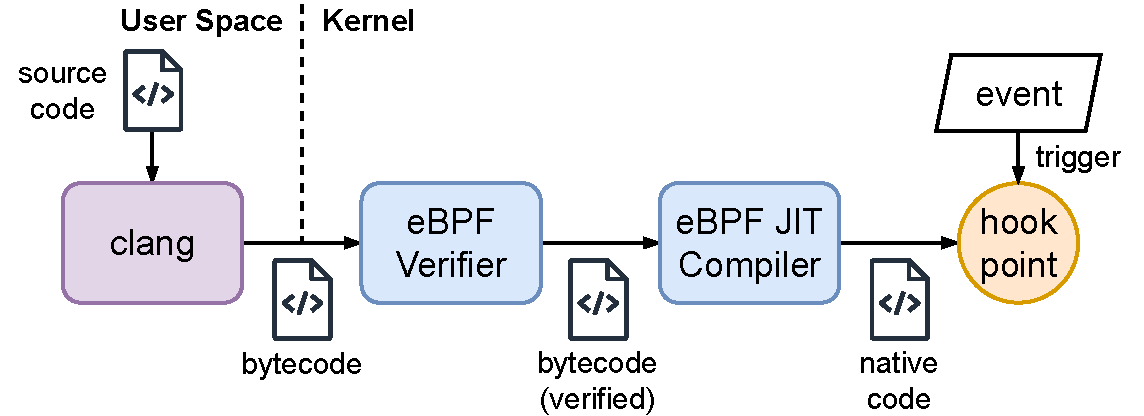
\includegraphics[width=\linewidth]{figures/sec-2-ebpf-pipeline.pdf}
  \caption{The eBPF execution pipeline.}
  \label{fig:ebpf}
\end{figure}

\noindent\textbf{Verifier.}
The eBPF verifier statically checks every loaded program for safety before the kernel runs the program. Specifically, the verifier proves properties such as memory safety, termination, and absence of uninitialized reads. The analysis uses abstract interpretation~\cite{gershuni2019simple} across all reachable execution paths, maintaining an abstract state for each register. Each of the 123 \note{double check RFCs} opcodes in the eBPF ISA~\cite{rfc9669} has a transfer function specifying how the opcode transforms the tracked state. Adding a new opcode therefore requires a new transfer function.

\noindent\textbf{JIT compiler.}
The eBPF JIT compiler translates the verified bytecode into native machine code. The translation proceeds one instruction at a time, with eBPF registers \texttt{r0}--\texttt{r10} mapped to predetermined native registers on each target architecture. Within each instruction, the JIT applies encoding-level optimizations such as selecting the shortest immediate encoding and choosing short jumps when the offset fits. The JIT performs none of the cross-instruction optimizations standard in mainstream compilers, such as global register allocation and instruction scheduling.

Both the eBPF verifier and the eBPF JIT operate on the same bytecode. Each component works at opcode granularity: the verifier applies a transfer function to each opcode, and the JIT compiles each opcode in isolation. Every new opcode in the ISA therefore requires corresponding logic in both the verifier and the JIT. Other bytecode systems arrange this verification-execution coupling differently.

\subsection{Bytecode Design in Related Systems}
\label{subsec:bytecode}

Several other systems compile source code to a bytecode that is then verified and translated to native machine code. LLVM~\cite{lattner2004llvm} is a compiler infrastructure for C, C++, and Rust that lowers source code to an IR in static single-assignment (SSA) form, optimizes the IR, and emits native code. The Java Virtual Machine (JVM)~\cite{lindholm2012jvms} executes programs through a stack-based bytecode, verified for type safety and JIT-compiled by HotSpot~\cite{paleczny2001java}. WebAssembly (Wasm)~\cite{haas2017bringing} is a portable bytecode for web browsers and embedded runtimes, validated at load time and compiled to native code.

These systems differ from eBPF in two respects, summarized in Table~\ref{tab:bytecode-comparison}. The first is how tightly verification constrains the ISA. LLVM imposes no safety verification on its IR; the backend is free to select any native instruction. Wasm validation checks control-flow structure and operand types, which constrains the ISA but still permits additions like single instruction, multiple data (SIMD) operations. The JVM verifier checks type safety per instruction, coupling verification to the bytecode at the granularity of individual opcodes. The eBPF verifier goes further than any of these, performing per-opcode abstract interpretation that tracks register types, value ranges, and memory provenance. Every new opcode therefore requires a matching transfer function (\S\ref{subsec:ebpf}). Among these systems, eBPF couples verification to the ISA at the finest granularity.

\begin{table}[t]
\centering
\small
\caption{Comparison of bytecode systems by verification requirements and optimization scope.}
\label{tab:bytecode-comparison}
\begin{tabular}{@{}lll@{}}
\toprule
System & Per-opcode verification & Optimization scope \\
\midrule
LLVM & None & Full \\
JVM & Type rules & Full \\
Wasm & Type + structural rules & Cross-instruction \\
eBPF & Abstract transfer function & Per-instruction \\
\bottomrule
\end{tabular}
\end{table}


The second is the scope of optimization in the compiler or JIT. LLVM runs a full optimization pipeline: register allocation, instruction selection, and instruction scheduling. The JVM's HotSpot C2 compiler uses a more complex JIT stack than the eBPF JIT compiler, including tiered compilation and aggressive optimization machinery. Wasm JIT engines also perform cross-instruction optimization, though at lower complexity than HotSpot. The eBPF JIT compiler optimizes the encoding of each instruction individually (e.g., shortest immediate, short jumps) but performs no cross-instruction optimization.

In LLVM, JVM, and Wasm, at least one of these two factors works in the system's favor: either verification is light enough that the ISA can be expressive, or the JIT performs cross-instruction optimization to compensate. eBPF is the only system among these four where verification is at its tightest and the JIT is limited to per-instruction encoding.

\subsection{Formal Verification of eBPF Components}
\label{subsec:formal}

Both the eBPF verifier and JIT have received formal verification. Jitterbug~\cite{nelson2020specification} verifies eBPF JIT correctness via SMT-based symbolic verification and found 16 previously unknown bugs across multiple architecture backends. Agni~\cite{vishwanathan2023verifying} applies symbolic verification to the verifier's range-analysis operators and found 27 bugs. 
% across 16 kernel versions. 
SEV~\cite{sun2024validating} validates the verifier's abstract approximations against concrete executions via state embedding and found 15 logic bugs.

Each of eBPF's formal verification proofs relies on the current verifier and JIT architecture. Jitterbug assumes the JIT translates one source instruction at a time, a property that holds for every in-kernel eBPF JIT. Agni and SEV verify the verifier's current abstract-interpretation structure.